\documentclass[twoside]{book}

% Packages required by doxygen
\usepackage{fixltx2e}
\usepackage{calc}
\usepackage{doxygen}
\usepackage[export]{adjustbox} % also loads graphicx
\usepackage{graphicx}
\usepackage[utf8]{inputenc}
\usepackage{makeidx}
\usepackage{multicol}
\usepackage{multirow}
\PassOptionsToPackage{warn}{textcomp}
\usepackage{textcomp}
\usepackage[nointegrals]{wasysym}
\usepackage[table]{xcolor}

% Font selection
\usepackage[T1]{fontenc}
\usepackage[scaled=.90]{helvet}
\usepackage{courier}
\usepackage{amssymb}
\usepackage{sectsty}
\renewcommand{\familydefault}{\sfdefault}
\allsectionsfont{%
  \fontseries{bc}\selectfont%
  \color{darkgray}%
}
\renewcommand{\DoxyLabelFont}{%
  \fontseries{bc}\selectfont%
  \color{darkgray}%
}
\newcommand{\+}{\discretionary{\mbox{\scriptsize$\hookleftarrow$}}{}{}}

% Page & text layout
\usepackage{geometry}
\geometry{%
  a4paper,%
  top=2.5cm,%
  bottom=2.5cm,%
  left=2.5cm,%
  right=2.5cm%
}
\tolerance=750
\hfuzz=15pt
\hbadness=750
\setlength{\emergencystretch}{15pt}
\setlength{\parindent}{0cm}
\setlength{\parskip}{3ex plus 2ex minus 2ex}
\makeatletter
\renewcommand{\paragraph}{%
  \@startsection{paragraph}{4}{0ex}{-1.0ex}{1.0ex}{%
    \normalfont\normalsize\bfseries\SS@parafont%
  }%
}
\renewcommand{\subparagraph}{%
  \@startsection{subparagraph}{5}{0ex}{-1.0ex}{1.0ex}{%
    \normalfont\normalsize\bfseries\SS@subparafont%
  }%
}
\makeatother

% Headers & footers
\usepackage{fancyhdr}
\pagestyle{fancyplain}
\fancyhead[LE]{\fancyplain{}{\bfseries\thepage}}
\fancyhead[CE]{\fancyplain{}{}}
\fancyhead[RE]{\fancyplain{}{\bfseries\leftmark}}
\fancyhead[LO]{\fancyplain{}{\bfseries\rightmark}}
\fancyhead[CO]{\fancyplain{}{}}
\fancyhead[RO]{\fancyplain{}{\bfseries\thepage}}
\fancyfoot[LE]{\fancyplain{}{}}
\fancyfoot[CE]{\fancyplain{}{}}
\fancyfoot[RE]{\fancyplain{}{\bfseries\scriptsize Generated by Doxygen }}
\fancyfoot[LO]{\fancyplain{}{\bfseries\scriptsize Generated by Doxygen }}
\fancyfoot[CO]{\fancyplain{}{}}
\fancyfoot[RO]{\fancyplain{}{}}
\renewcommand{\footrulewidth}{0.4pt}
\renewcommand{\chaptermark}[1]{%
  \markboth{#1}{}%
}
\renewcommand{\sectionmark}[1]{%
  \markright{\thesection\ #1}%
}

% Indices & bibliography
\usepackage{natbib}
\usepackage[titles]{tocloft}
\setcounter{tocdepth}{3}
\setcounter{secnumdepth}{5}
\makeindex

% Hyperlinks (required, but should be loaded last)
\usepackage{ifpdf}
\ifpdf
  \usepackage[pdftex,pagebackref=true]{hyperref}
\else
  \usepackage[ps2pdf,pagebackref=true]{hyperref}
\fi
\hypersetup{%
  colorlinks=true,%
  linkcolor=blue,%
  citecolor=blue,%
  unicode%
}

% Custom commands
\newcommand{\clearemptydoublepage}{%
  \newpage{\pagestyle{empty}\cleardoublepage}%
}

\usepackage{caption}
\captionsetup{labelsep=space,justification=centering,font={bf},singlelinecheck=off,skip=4pt,position=top}

%===== C O N T E N T S =====

\begin{document}

% Titlepage & ToC
\hypersetup{pageanchor=false,
             bookmarksnumbered=true,
             pdfencoding=unicode
            }
\pagenumbering{alph}
\begin{titlepage}
\vspace*{7cm}
\begin{center}%
{\Large D\+A\+GS }\\
\vspace*{1cm}
{\large Generated by Doxygen 1.8.13}\\
\end{center}
\end{titlepage}
\clearemptydoublepage
\pagenumbering{roman}
\tableofcontents
\clearemptydoublepage
\pagenumbering{arabic}
\hypersetup{pageanchor=true}

%--- Begin generated contents ---
\chapter{Data Structure Index}
\section{Data Structures}
Here are the data structures with brief descriptions\+:\begin{DoxyCompactList}
\item\contentsline{section}{\hyperlink{structAES256__CTR__DRBG__struct}{A\+E\+S256\+\_\+\+C\+T\+R\+\_\+\+D\+R\+B\+G\+\_\+struct} }{\pageref{structAES256__CTR__DRBG__struct}}{}
\item\contentsline{section}{\hyperlink{structAES__XOF__struct}{A\+E\+S\+\_\+\+X\+O\+F\+\_\+struct} }{\pageref{structAES__XOF__struct}}{}
\item\contentsline{section}{\hyperlink{structmatrix}{matrix} }{\pageref{structmatrix}}{}
\item\contentsline{section}{\hyperlink{structpolynome}{polynome} }{\pageref{structpolynome}}{}
\end{DoxyCompactList}

\chapter{File Index}
\section{File List}
Here is a list of all documented files with brief descriptions\+:\begin{DoxyCompactList}
\item\contentsline{section}{src/{\bfseries api.\+h} }{\pageref{api_8h}}{}
\item\contentsline{section}{src/{\bfseries cycles.\+h} }{\pageref{cycles_8h}}{}
\item\contentsline{section}{src/{\bfseries decapsulation.\+h} }{\pageref{decapsulation_8h}}{}
\item\contentsline{section}{src/{\bfseries decoding.\+h} }{\pageref{decoding_8h}}{}
\item\contentsline{section}{src/{\bfseries encapsulation.\+h} }{\pageref{encapsulation_8h}}{}
\item\contentsline{section}{src/{\bfseries fichier.\+h} }{\pageref{fichier_8h}}{}
\item\contentsline{section}{src/{\bfseries gf.\+h} }{\pageref{gf_8h}}{}
\item\contentsline{section}{src/{\bfseries keccak\+\_\+f.\+h} }{\pageref{keccak__f_8h}}{}
\item\contentsline{section}{src/\hyperlink{key__gen_8h}{key\+\_\+gen.\+h} \\*File that contains the key pair generation }{\pageref{key__gen_8h}}{}
\item\contentsline{section}{src/{\bfseries matrix.\+h} }{\pageref{matrix_8h}}{}
\item\contentsline{section}{src/{\bfseries param.\+h} }{\pageref{param_8h}}{}
\item\contentsline{section}{src/{\bfseries poly.\+h} }{\pageref{poly_8h}}{}
\item\contentsline{section}{src/{\bfseries rng.\+h} }{\pageref{rng_8h}}{}
\item\contentsline{section}{src/{\bfseries round.\+h} }{\pageref{round_8h}}{}
\item\contentsline{section}{src/{\bfseries sponge.\+h} }{\pageref{sponge_8h}}{}
\item\contentsline{section}{src/{\bfseries util.\+h} }{\pageref{util_8h}}{}
\end{DoxyCompactList}

\chapter{Data Structure Documentation}
\hypertarget{structAES256__CTR__DRBG__struct}{}\section{A\+E\+S256\+\_\+\+C\+T\+R\+\_\+\+D\+R\+B\+G\+\_\+struct Struct Reference}
\label{structAES256__CTR__DRBG__struct}\index{A\+E\+S256\+\_\+\+C\+T\+R\+\_\+\+D\+R\+B\+G\+\_\+struct@{A\+E\+S256\+\_\+\+C\+T\+R\+\_\+\+D\+R\+B\+G\+\_\+struct}}
\subsection*{Data Fields}
\begin{DoxyCompactItemize}
\item 
\mbox{\Hypertarget{structAES256__CTR__DRBG__struct_a9e6db229bc3b894fd8d647367b2bbd9f}\label{structAES256__CTR__DRBG__struct_a9e6db229bc3b894fd8d647367b2bbd9f}} 
unsigned char {\bfseries Key} \mbox{[}32\mbox{]}
\item 
\mbox{\Hypertarget{structAES256__CTR__DRBG__struct_a4f688fb7ba4142ae56d4aaa58f508f03}\label{structAES256__CTR__DRBG__struct_a4f688fb7ba4142ae56d4aaa58f508f03}} 
unsigned char {\bfseries V} \mbox{[}16\mbox{]}
\item 
\mbox{\Hypertarget{structAES256__CTR__DRBG__struct_ad134015fd195406e6403e70bb108839c}\label{structAES256__CTR__DRBG__struct_ad134015fd195406e6403e70bb108839c}} 
int {\bfseries reseed\+\_\+counter}
\end{DoxyCompactItemize}


The documentation for this struct was generated from the following file\+:\begin{DoxyCompactItemize}
\item 
src/rng.\+h\end{DoxyCompactItemize}

\hypertarget{structAES__XOF__struct}{}\section{A\+E\+S\+\_\+\+X\+O\+F\+\_\+struct Struct Reference}
\label{structAES__XOF__struct}\index{A\+E\+S\+\_\+\+X\+O\+F\+\_\+struct@{A\+E\+S\+\_\+\+X\+O\+F\+\_\+struct}}
\subsection*{Data Fields}
\begin{DoxyCompactItemize}
\item 
\mbox{\Hypertarget{structAES__XOF__struct_a0dccd2463f4520272e9c7cde8a9a1cc1}\label{structAES__XOF__struct_a0dccd2463f4520272e9c7cde8a9a1cc1}} 
unsigned char {\bfseries buffer} \mbox{[}16\mbox{]}
\item 
\mbox{\Hypertarget{structAES__XOF__struct_a04e9673c4aa42b5de3c4bc21e640544c}\label{structAES__XOF__struct_a04e9673c4aa42b5de3c4bc21e640544c}} 
int {\bfseries buffer\+\_\+pos}
\item 
\mbox{\Hypertarget{structAES__XOF__struct_a4400350c04e5e05c124b8e7a42d51aab}\label{structAES__XOF__struct_a4400350c04e5e05c124b8e7a42d51aab}} 
unsigned long {\bfseries length\+\_\+remaining}
\item 
\mbox{\Hypertarget{structAES__XOF__struct_af6c77acc5b67da8a5d9424022a6801c7}\label{structAES__XOF__struct_af6c77acc5b67da8a5d9424022a6801c7}} 
unsigned char {\bfseries key} \mbox{[}32\mbox{]}
\item 
\mbox{\Hypertarget{structAES__XOF__struct_abddd02f31b49f037543ee2726eae552b}\label{structAES__XOF__struct_abddd02f31b49f037543ee2726eae552b}} 
unsigned char {\bfseries ctr} \mbox{[}16\mbox{]}
\end{DoxyCompactItemize}


The documentation for this struct was generated from the following file\+:\begin{DoxyCompactItemize}
\item 
src/rng.\+h\end{DoxyCompactItemize}

\hypertarget{structmatrix}{}\section{matrix Struct Reference}
\label{structmatrix}\index{matrix@{matrix}}
\subsection*{Data Fields}
\begin{DoxyCompactItemize}
\item 
\mbox{\Hypertarget{structmatrix_a0e6b7009d531ba82b3de92abd90114a3}\label{structmatrix_a0e6b7009d531ba82b3de92abd90114a3}} 
unsigned int {\bfseries rown}
\item 
\mbox{\Hypertarget{structmatrix_a2a80e12fe066ce9cafc0527b562dd270}\label{structmatrix_a2a80e12fe066ce9cafc0527b562dd270}} 
unsigned int {\bfseries coln}
\item 
\mbox{\Hypertarget{structmatrix_a1684926400668b59acc7ac6863729441}\label{structmatrix_a1684926400668b59acc7ac6863729441}} 
gf $\ast$$\ast$ {\bfseries coeff}
\end{DoxyCompactItemize}


The documentation for this struct was generated from the following file\+:\begin{DoxyCompactItemize}
\item 
src/matrix.\+h\end{DoxyCompactItemize}

\hypertarget{structpolynome}{}\section{polynome Struct Reference}
\label{structpolynome}\index{polynome@{polynome}}
\subsection*{Data Fields}
\begin{DoxyCompactItemize}
\item 
\mbox{\Hypertarget{structpolynome_a5feaa681dce2b731eabc1681f9a3e097}\label{structpolynome_a5feaa681dce2b731eabc1681f9a3e097}} 
int {\bfseries deg}
\item 
\mbox{\Hypertarget{structpolynome_a4d9c64324a05ff23bff85eaf192162d1}\label{structpolynome_a4d9c64324a05ff23bff85eaf192162d1}} 
int {\bfseries size}
\item 
\mbox{\Hypertarget{structpolynome_a3bf33057f1e26dff82f49ece722e2a75}\label{structpolynome_a3bf33057f1e26dff82f49ece722e2a75}} 
gf $\ast$ {\bfseries coeff}
\end{DoxyCompactItemize}


The documentation for this struct was generated from the following file\+:\begin{DoxyCompactItemize}
\item 
src/poly.\+h\end{DoxyCompactItemize}

\chapter{File Documentation}
\hypertarget{key__gen_8h}{}\section{src/key\+\_\+gen.h File Reference}
\label{key__gen_8h}\index{src/key\+\_\+gen.\+h@{src/key\+\_\+gen.\+h}}


File that contains the key pair generation.  


{\ttfamily \#include $<$stdio.\+h$>$}\newline
{\ttfamily \#include $<$stdlib.\+h$>$}\newline
{\ttfamily \#include $<$string.\+h$>$}\newline
{\ttfamily \#include $<$time.\+h$>$}\newline
{\ttfamily \#include $<$math.\+h$>$}\newline
{\ttfamily \#include \char`\"{}decoding.\+h\char`\"{}}\newline
{\ttfamily \#include \char`\"{}matrix.\+h\char`\"{}}\newline
{\ttfamily \#include \char`\"{}fichier.\+h\char`\"{}}\newline
{\ttfamily \#include \char`\"{}poly.\+h\char`\"{}}\newline
{\ttfamily \#include \char`\"{}param.\+h\char`\"{}}\newline
{\ttfamily \#include \char`\"{}util.\+h\char`\"{}}\newline
{\ttfamily \#include \char`\"{}rng.\+h\char`\"{}}\newline
Include dependency graph for key\+\_\+gen.\+h\+:\nopagebreak
\begin{figure}[H]
\begin{center}
\leavevmode
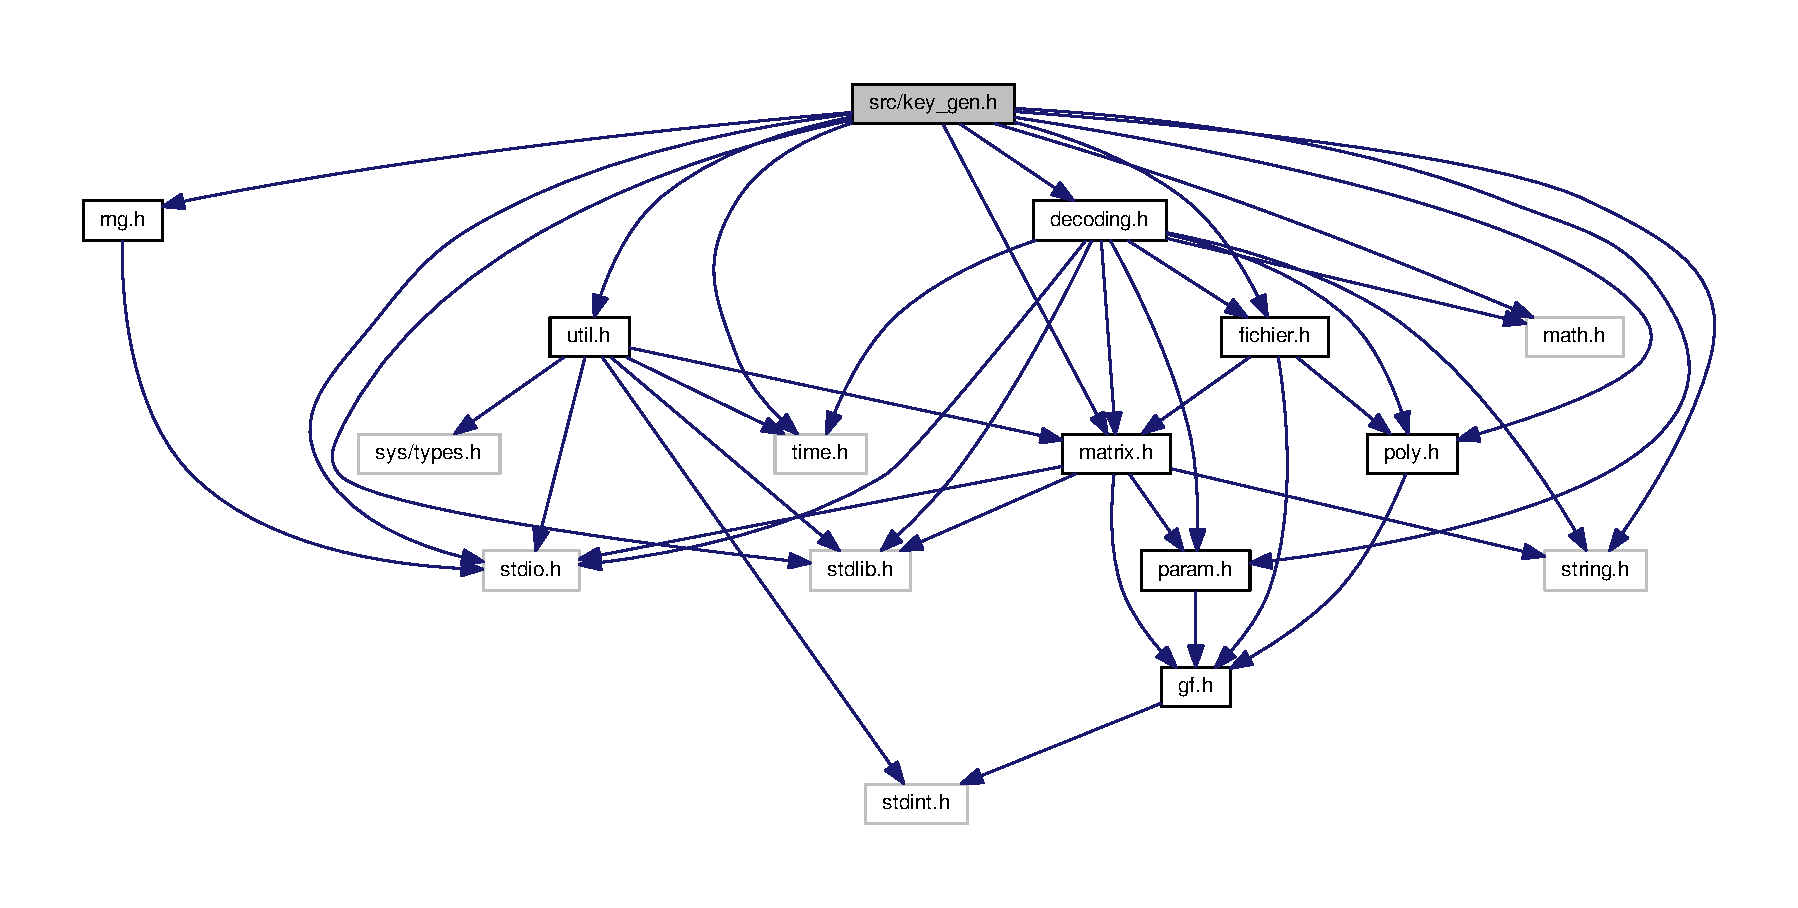
\includegraphics[width=350pt]{key__gen_8h__incl}
\end{center}
\end{figure}
\subsection*{Functions}
\begin{DoxyCompactItemize}
\item 
int \hyperlink{key__gen_8h_abd18ce43e4be62524154e3ba889d0840}{disjoint\+\_\+test} (gf $\ast$u, gf $\ast$v)
\begin{DoxyCompactList}\small\item\em check if the vectors are disjoint \end{DoxyCompactList}\item 
void \hyperlink{key__gen_8h_a528780956a7c8358c007982fe6653880}{generate\+\_\+random\+\_\+vector} (int m, gf $\ast$vect)
\begin{DoxyCompactList}\small\item\em Method to generate a random vector. \end{DoxyCompactList}\item 
void \hyperlink{key__gen_8h_a5baf3fca90a4cff6e17756eabb4b63b0}{init\+\_\+random\+\_\+element} (gf $\ast$U)
\begin{DoxyCompactList}\small\item\em Method to initialize a vector. \end{DoxyCompactList}\item 
void \hyperlink{key__gen_8h_a3017dc4a6e1c902b1477aeb7caa0695d}{binary\+\_\+quasi\+\_\+dyadic\+\_\+sig} (int m, int n, int t, int $\ast$b, gf $\ast$h\+\_\+sig, gf $\ast$w)
\begin{DoxyCompactList}\small\item\em Binary quasi dyadic signature. \end{DoxyCompactList}\item 
void \hyperlink{key__gen_8h_a3209fb803bf98f133faf4ec56030cc5d}{cauchy\+\_\+support} (gf $\ast$support, gf $\ast$u, gf $\ast$w)
\begin{DoxyCompactList}\small\item\em Binary Cauchy support. \end{DoxyCompactList}\item 
int \hyperlink{key__gen_8h_a42acf0c4407e29a615aef53a4dd45952}{key\+\_\+pair} (unsigned char $\ast$pk, unsigned char $\ast$sk)
\begin{DoxyCompactList}\small\item\em Key pair generation. \end{DoxyCompactList}\end{DoxyCompactItemize}


\subsection{Detailed Description}
File that contains the key pair generation. 

The file contains the key generation elements, i.\+e, The quasi-\/dyadic-\/signature and cauchy support generation. 

\subsection{Function Documentation}
\mbox{\Hypertarget{key__gen_8h_a3017dc4a6e1c902b1477aeb7caa0695d}\label{key__gen_8h_a3017dc4a6e1c902b1477aeb7caa0695d}} 
\index{key\+\_\+gen.\+h@{key\+\_\+gen.\+h}!binary\+\_\+quasi\+\_\+dyadic\+\_\+sig@{binary\+\_\+quasi\+\_\+dyadic\+\_\+sig}}
\index{binary\+\_\+quasi\+\_\+dyadic\+\_\+sig@{binary\+\_\+quasi\+\_\+dyadic\+\_\+sig}!key\+\_\+gen.\+h@{key\+\_\+gen.\+h}}
\subsubsection{\texorpdfstring{binary\+\_\+quasi\+\_\+dyadic\+\_\+sig()}{binary\_quasi\_dyadic\_sig()}}
{\footnotesize\ttfamily void binary\+\_\+quasi\+\_\+dyadic\+\_\+sig (\begin{DoxyParamCaption}\item[{int}]{m,  }\item[{int}]{n,  }\item[{int}]{t,  }\item[{int $\ast$}]{b,  }\item[{gf $\ast$}]{h\+\_\+sig,  }\item[{gf $\ast$}]{w }\end{DoxyParamCaption})}



Binary quasi dyadic signature. 


\begin{DoxyParams}{Parameters}
{\em m} & size of code word. \\
\hline
{\em n} & value to check when stop at the first non-\/zero element of V. \\
\hline
{\em t} & \\
\hline
{\em b} & auxiliar. \\
\hline
{\em h\+\_\+sig} & element that will receive the signature. \\
\hline
{\em w} & element to be signed. \\
\hline
\end{DoxyParams}
\mbox{\Hypertarget{key__gen_8h_a3209fb803bf98f133faf4ec56030cc5d}\label{key__gen_8h_a3209fb803bf98f133faf4ec56030cc5d}} 
\index{key\+\_\+gen.\+h@{key\+\_\+gen.\+h}!cauchy\+\_\+support@{cauchy\+\_\+support}}
\index{cauchy\+\_\+support@{cauchy\+\_\+support}!key\+\_\+gen.\+h@{key\+\_\+gen.\+h}}
\subsubsection{\texorpdfstring{cauchy\+\_\+support()}{cauchy\_support()}}
{\footnotesize\ttfamily void cauchy\+\_\+support (\begin{DoxyParamCaption}\item[{gf $\ast$}]{support,  }\item[{gf $\ast$}]{u,  }\item[{gf $\ast$}]{w }\end{DoxyParamCaption})}



Binary Cauchy support. 


\begin{DoxyParams}{Parameters}
{\em support} & element to be the support \\
\hline
{\em u} & input vector to be used \\
\hline
{\em w} & input vector to be used \\
\hline
\end{DoxyParams}
\mbox{\Hypertarget{key__gen_8h_abd18ce43e4be62524154e3ba889d0840}\label{key__gen_8h_abd18ce43e4be62524154e3ba889d0840}} 
\index{key\+\_\+gen.\+h@{key\+\_\+gen.\+h}!disjoint\+\_\+test@{disjoint\+\_\+test}}
\index{disjoint\+\_\+test@{disjoint\+\_\+test}!key\+\_\+gen.\+h@{key\+\_\+gen.\+h}}
\subsubsection{\texorpdfstring{disjoint\+\_\+test()}{disjoint\_test()}}
{\footnotesize\ttfamily int disjoint\+\_\+test (\begin{DoxyParamCaption}\item[{gf $\ast$}]{u,  }\item[{gf $\ast$}]{v }\end{DoxyParamCaption})}



check if the vectors are disjoint 


\begin{DoxyParams}{Parameters}
{\em u} & -\/ input vector. \\
\hline
{\em v} & -\/ the other vector to check.\\
\hline
\end{DoxyParams}
\begin{DoxyReturn}{Returns}


if it is disjoint it will be 0 if not wil return -\/1. 
\end{DoxyReturn}
\mbox{\Hypertarget{key__gen_8h_a528780956a7c8358c007982fe6653880}\label{key__gen_8h_a528780956a7c8358c007982fe6653880}} 
\index{key\+\_\+gen.\+h@{key\+\_\+gen.\+h}!generate\+\_\+random\+\_\+vector@{generate\+\_\+random\+\_\+vector}}
\index{generate\+\_\+random\+\_\+vector@{generate\+\_\+random\+\_\+vector}!key\+\_\+gen.\+h@{key\+\_\+gen.\+h}}
\subsubsection{\texorpdfstring{generate\+\_\+random\+\_\+vector()}{generate\_random\_vector()}}
{\footnotesize\ttfamily void generate\+\_\+random\+\_\+vector (\begin{DoxyParamCaption}\item[{int}]{m,  }\item[{gf $\ast$}]{vect }\end{DoxyParamCaption})}



Method to generate a random vector. 


\begin{DoxyParams}{Parameters}
{\em m} & size of random bits. \\
\hline
{\em vect} & pointer that will be written the bits. \\
\hline
\end{DoxyParams}
\mbox{\Hypertarget{key__gen_8h_a5baf3fca90a4cff6e17756eabb4b63b0}\label{key__gen_8h_a5baf3fca90a4cff6e17756eabb4b63b0}} 
\index{key\+\_\+gen.\+h@{key\+\_\+gen.\+h}!init\+\_\+random\+\_\+element@{init\+\_\+random\+\_\+element}}
\index{init\+\_\+random\+\_\+element@{init\+\_\+random\+\_\+element}!key\+\_\+gen.\+h@{key\+\_\+gen.\+h}}
\subsubsection{\texorpdfstring{init\+\_\+random\+\_\+element()}{init\_random\_element()}}
{\footnotesize\ttfamily void init\+\_\+random\+\_\+element (\begin{DoxyParamCaption}\item[{gf $\ast$}]{U }\end{DoxyParamCaption})}



Method to initialize a vector. 


\begin{DoxyParams}{Parameters}
{\em U} & vector that will be initialize. \\
\hline
\end{DoxyParams}
\mbox{\Hypertarget{key__gen_8h_a42acf0c4407e29a615aef53a4dd45952}\label{key__gen_8h_a42acf0c4407e29a615aef53a4dd45952}} 
\index{key\+\_\+gen.\+h@{key\+\_\+gen.\+h}!key\+\_\+pair@{key\+\_\+pair}}
\index{key\+\_\+pair@{key\+\_\+pair}!key\+\_\+gen.\+h@{key\+\_\+gen.\+h}}
\subsubsection{\texorpdfstring{key\+\_\+pair()}{key\_pair()}}
{\footnotesize\ttfamily int key\+\_\+pair (\begin{DoxyParamCaption}\item[{unsigned char $\ast$}]{pk,  }\item[{unsigned char $\ast$}]{sk }\end{DoxyParamCaption})}



Key pair generation. 


\begin{DoxyParams}{Parameters}
{\em pk} & string that will be stored the public key \\
\hline
{\em sk} & string that will be sotred the secret key\\
\hline
\end{DoxyParams}
\begin{DoxyReturn}{Returns}
It will back 0 if it was possible to generate both keys and it will return != 0 if it wasn\textquotesingle{}t possible to generate keys. 
\end{DoxyReturn}

%--- End generated contents ---

% Index
\backmatter
\newpage
\phantomsection
\clearemptydoublepage
\addcontentsline{toc}{chapter}{Index}
\printindex

\end{document}
